\documentclass[spanish]{beamer}
\usepackage[utf8]{inputenc}
\usepackage{float}
\usepackage{beamerthemesplit}
\usepackage{latexsym}
\usepackage[T1]{fontenc}
\usepackage{amsmath}
\usepackage{hyperref}
\usepackage{graphicx}
\usepackage{babel,blindtext}
\usepackage{amsfonts}
\usepackage[round]{natbib}
\bibliographystyle{chicago}
\usepackage{subcaption} 


\decimalpoint

\usetheme{Antibes}%este es el templete que se usa a lo largo de la presentacion
%themes
%   default
%   Boadilla
%   Madrid
%   Pittsburgh
%   Copenhagen
%   Warsaw
%   Singapore
%   Malmoe
\newcommand\Fontvi{\fontsize{6}{7.2}\selectfont}
\mode<presentation>%tipo de 
\begin{document}

%%%%%%%%%%%%%%%%%%%%%%%%%%%%%%%%%%%%%%%%%%%%%%%%%%%%%%%%%%%%%%%%%%%%%%%%%%%%%%%%%%%%%%%%%%%%%%%%%%%%%%%%%%%%%
\title{Introducción a Procesos Estocásticos}
\author{Gamaliel Moreno Chávez}
\institute{MCPI}
\date{Ago-Dic\\ 2020}%para que ponga la fecha de hoy 

\frame{\titlepage}
%%%%%%%%%%%%%%%%%%%%%%%%%%%%%%%%%%%%%%%%%%%%%%%%%%%%%%%%%%%%%%%%%%%%%%%%%%%%%%%%%%%%%%%%%%%%%%%%%%%%%%%%%%%%%
%%%%%%%%%%%%%%%%%%%%%%%%%%%%%%%%%%%%%%%%%%%%%%%%%%%%%%%%%%%%%%%%%%%%%%%%%%%%%%%%%%%%%%%%%%%%%%%%%%%%%%%%%%%%%%%%%%%%%%%%%%%%%%%%%%%%%%%%%%%%%%%%%%%%%%%%%%%%%%%%%%%%%%%%%%%%%%%%%%%%%%%%%%%%%%%%%%%%%%%%%%%%%%%%%%%%%%%%%%
%%%%%%%%%%%%%%%%%%%%%%%%%%%%%%%%%%%%%%%%%%%%%%%%%%%%%%%%%%%%%%%%%%%%%%%%%%%%%%%%%%%%%%%%%%%%%%%%%%%%%%%%%%%%%%%%%%%%%%%%%%%%%%%%%%%%%%%%%%%%%%%%%%%%%%%%%%%%%%%%%%%%%%%%%%%%%%%%%%%%%%%%%%%%%%%%%%%%%%%%%%%%%%%%%%%%%%%%%%

\begin{frame}
\frametitle{Generalidades}
La estadística y la probabilidad nacieron juntas pero son ciencias diferentes. 

\begin{center}
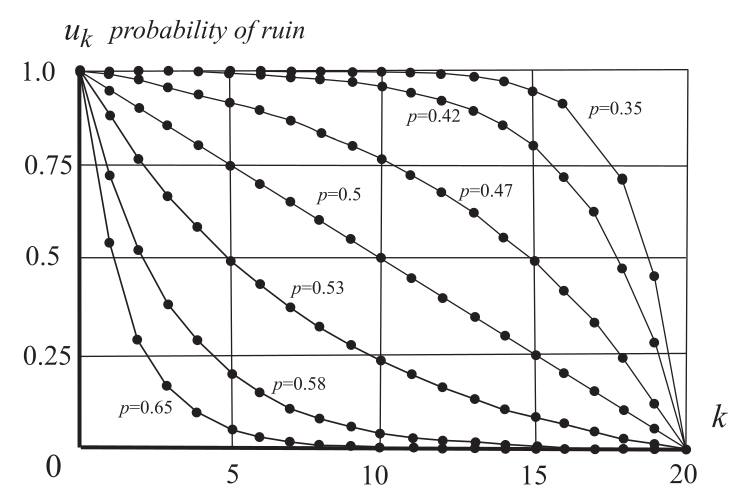
\includegraphics[scale=0.9]{im1}
\end{center}

Racionalidad limitada. No se tiene toda la información. No se puede procesar toda la información.  
\end{frame}

%%%%%%%%%%%%%%%%%%%%%%%%%%%%%%%%%%%%%%%%%%%%%%%%%%%%%%%%%%%%%%%%%%%%%%%%%%%%%%%%%%%%%%%%%%%%%%%%%%%%%%%%%%%%%
\begin{frame}
\frametitle{Determinismo} 
 \begin{itemize}
 \item El resultado del modelo es investigado por las condiciones iniciales y los parámetros.
 \item Sistema BIBO para modelos lineales bien definidos y multiples salidas para sistemas no lineales.
 \item Modelos pueden ser descritos en diferentes niveles de variación temporal, estado estacionario (independencia temporal), estado no estacionario (dependencia temporal) y dinámica. 
 \end{itemize}
\end{frame}
%%%%%%%%%%%%%%%%%%%%%%%%%%%%%%%%%%%%%%%%%%%%%%%%%%%%%%%%%%%%%%%%%%%%%%%%%%%%%%%%%%%%%%%%%%%%%%%%%%%%%%%%%%%%%
\begin{frame}
\frametitle{Estocástico}
 \begin{itemize}
 \item Los procesos tiene una aleatoriedad inherente, así que, el mismo conjunto de valores y parámetros iniciales producen diferentes salidas. 
  
 \item Los modelos estocásticos toman en cuenta incertidumbres causadas por la variación del comportamiento. Por lo tanto, se puede decir que esto es más informativo que los determinísticos. 

 \end{itemize}

\end{frame}
%%%%%%%%%%%%%%%%%%%%%%%%%%%%%%%%%%%%%%%%%%%%%%%%%%%%%%%%%%%%%%%%%%%%%%%%%%%%%%%%%%%%%%%%%%%%%%%%%%%%%%%%%%%%%
\begin{frame}
\frametitle{Procesos estocásticos}
\begin{center}
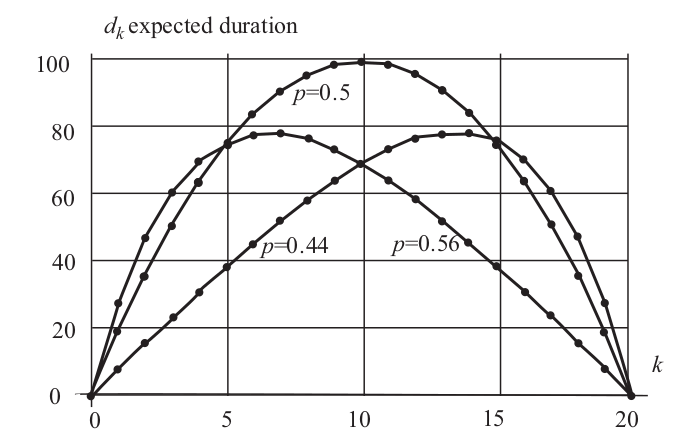
\includegraphics[scale=0.4]{im2}
\end{center}
\end{frame}
%%%%%%%%%%%%%%%%%%%%%%%%%%%%%%%%%%%%%%%%%%%%%%%%%%%%%%%%%%%%%%%%%%%%%%%%%%%%%%%%%%%%%%%%%%%%%%%%%%%%%%%%%%%%%
\begin{frame}
\frametitle{Definición}
\begin{itemize}
\item Un proceso estocástico es una colección infinita de variables aleatorias (v.a.s.)
\item $X_{t} =$ ''estado de un sistema al tiempo t"
\item $t\in T= \lbrace 1,2, \ldots \rbrace$ o $t\in T = [0,\infty \rbrace$ 
\item $X_{t} \in S  \subseteq = \mathfrak{R}$ 
\end{itemize}
\end{frame}
%%%%%%%%%%%%%%%%%%%%%%%%%%%%%%%%%%%%%%%%%%%%%%%%%%%%%%%%%%%%%%%%%%%%%%%%%%%%%%%%%%%%%%%%%%%%%%%%%%%%%%%%%%%%%
\begin{frame}
\frametitle{Definición}
\begin{block}{Definición formal de procesos estocástico}
Un proceso estocástico es una colección de v.a.s. $\lbrace x_{t}: t \in T \rbrace$ parametrizada por un conjunto T llamado espacio parametral, en donde las v.a.s. toman valores en un conjunto s llamado espacio de estados. 
\end{block}

\end{frame}
%%%%%%%%%%%%%%%%%%%%%%%%%%%%%%%%%%%%%%%%%%%%%%%%%%%%%%%%%%%%%%%%%%%%%%%%%%%%%%%%%%%%%%%%%%%%%%%%%%%%%%%%%%%%%
\begin{frame}
\frametitle{Procesos estocásticos}
\begin{center}
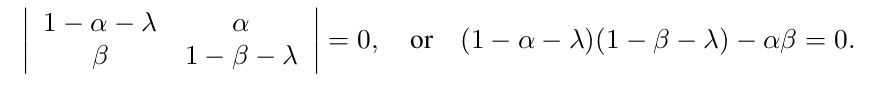
\includegraphics[scale=0.6]{im3}
\end{center}
\end{frame}
%%%%%%%%%%%%%%%%%%%%%%%%%%%%%%%%%%%%%%%%%%%%%%%%%%%%%%%%%%%%%%%%%%%%%%%%%%%%%%%%%%%%%%%%%%%%%%%%%%%%%%%%%%%%%
\begin{frame}
\frametitle{Procesos estocásticos}
\begin{itemize}
\item Para describir un proceso estocástico basta conocer la distribución de probabilidad conjunta de dichas variables.
\item Para cada $t$ el sistema se encuentra en uno de los estados mutuamente excluyentes; $0,1,2, \ldtos, M$
\item Si T es finito se trata de un procesos discreto 
\item Si T es un subconjunto de los reales se trata de un proceso continuo
\end{itemize}

\end{frame}
%%%%%%%%%%%%%%%%%%%%%%%%%%%%%%%%%%%%%%%%%%%%%%%%%%%%%%%%%%%%%%%%%%%%%%%%%%%%%%%%%%%%%%%%%%%%%%%%%%%%%%%%%%%%%
\begin{frame}
\frametitle{Tipos de procesos estocásticos}
\begin{enumerate}
\item Distintos espacios parametrales.
\item Distintos espacios de estado.
\item Distintas características de las trayectorias. 
\item Distintas relaciones de dependencia estocástica entre las v.a.s. que conforman el proceso
\end{enumerate}
\end{frame}

%%%%%%%%%%%%%%%%%%%%%%%%%%%%%%%%%%%%%%%%%%%%%%%%%%%%%%%%%%%%%%%%%%%%%%%%%%%%%%%%%%%%%%%%%%%%%%%%%%%%%%%%%%%%%
\end {document}



                                                  






